\documentclass[../../document.tex]{subfiles}
\begin{document}

\section*{Aufgabe 5}

\begin{figure}[H]
    \begin{center}
        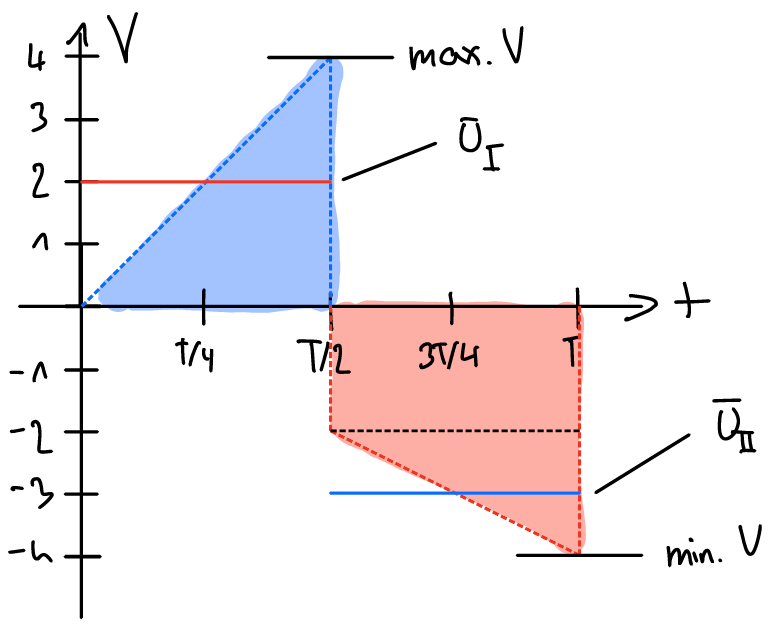
\includegraphics[width=.9\linewidth]{../../img/aufg5}
    \end{center}
\end{figure}

\subsection*{a) - Mittelwert}

\emph{Graphisch ermittelt}

\begin{equation*}
    \begin{split}
        \bar{U}\cind{I} &= \SI{2}{\volt}\\
        \bar{U}\cind{II} &= \SI{-3}{\volt}\\
        \bar{U} &= \frac{\bar{U}\cind{I} + \bar{U}\cind{II}}{2} = \SI{-0,5}{\volt}
    \end{split}
\end{equation*}

\newpage

\subsection*{b) - Effektivwert}

\emph{Formeln graphisch ermittelt}

\begin{equation*}
    \begin{split}
        U\cind{I} (t) &= \frac{\SI{8}{\volt}}{T} * t, 0 \leq t \leq \frac{T}{2}\\
        U\cind{II} (t) &= \frac{\SI{-4}{\volt}}{T} * t, \frac{T}{2} \leq t \leq T\\
    \end{split}
\end{equation*}

Allgemeine Berechnungsformel

\[U\cind{eff} = \sqrt{\frac{1}{T} \int_{0}^{T} u(t)^2 dt}\]

Integrale aufteilen (für jeden Abschnitt)

\[\Rightarrow U\cind{eff} = \sqrt{\frac{1}{T} ( \int_{0}^{\frac{T}{2}} ( \frac{\SI{8}{\volt}}{T} * t )^2 dt + \int_{\frac{T}{2}}^{T} (\frac{\SI{-4}{\volt}}{T} * t)^2 dt )}\]

Quadrierte Klammern auflösen

\[\Leftrightarrow U\cind{eff} = \sqrt{\frac{1}{T} ( \int_{0}^{\frac{T}{2}} \frac{\SI{64}{\volt^2}}{T^2} * t^2 dt + \int_{\frac{T}{2}}^{T} \frac{\SI{16}{\volt^2}}{T^2} * t^2 dt )}\]

Integrale auflösen

\[\Leftrightarrow U\cind{eff} = \sqrt{\frac{1}{T} ( \left[ \frac{\SI{64}{\volt^2}}{3T^2} * t^3 \right]_0^{\frac{T}{2}} + \left[ \frac{\SI{16}{\volt^2}}{3T^2} * t^3 \right]_{\frac{T}{2}}^{T} ) }\]

Grenzen der Integrale einsetzen und T kürzen

\[\Leftrightarrow U\cind{eff} = \sqrt{\frac{1}{T} ( \frac{\SI{64}{\volt^2}}{3T^2} * (\frac{T}{2})^2 + \frac{\SI{16}{\volt^2}}{3T^2} * T^3 - \frac{\SI{16}{\volt^2}}{3T^2} * (\frac{T}{2})^3 )} \]

Termumformung

\[\Leftrightarrow U\cind{eff} = \sqrt{\frac{1}{T} (\frac{\SI{64}{\volt^2T}}{24} + \frac{\SI{16}{\volt^2T}}{3} - \frac{\SI{16}{\volt^2T}}{24})} = \sqrt{\frac{\SI{22}{\volt^2}}{3}} = \frac{\sqrt{66}}{3}\SI{}{V}\]

\newpage

\subsection*{c) - Gleichrichtwert}

\emph{Graphisch ermittelt}

\begin{equation*}
    \begin{split}
        \left\lvert \bar{U}\cind{I} \right\rvert &= 2V\\
        \left\lvert \bar{U}\cind{II} \right\rvert &= 3V\\
        \left\lvert \bar{U} \right\rvert &= \frac{ \left\lvert \bar{U}\cind{I} \right\rvert + \left\lvert \bar{U}\cind{II} \right\rvert }{2} = \frac{\SI{5}{\volt}}{2} = \SI{2,5}{\volt}\\
    \end{split}
\end{equation*}

\end{document}